\documentclass[11pt,a4paper]{article}
\usepackage[utf8]{inputenc}
\usepackage{amsmath}
\usepackage{amsfonts}
\usepackage{amssymb}
\usepackage{graphicx}
\author{Battet, Bouhadana, Demimuid, Suong, Théate}
\title{Cahier des charges \\
\textbf {SmartKoulak}}
\begin{document}
\maketitle

\paragraph{}La gestion d'une exploitation agricole est une tâche complexe et chronophage. Les agriculteurs doivent en effet tenir compte de nombreux paramètres souvent peu précis et utiliser des méthodes empiriques pour assurer la qualité de leur exploitation, sans toutefois garantir l'optimalité des dépenses. Le projet \textit{SmartKoulak} vise à redonner aux agriculteurs un plein contrôle de leur exploitation.


\section{Présentation}
\paragraph{}Bien que l’agriculture existe depuis l’aube de l’humanité, ce secteur n’a connu de révolution majeure que récemment. Cependant malgré les évolutions technologiques la gestion des plantations reste une tâche complexe et difficilement automatisable. On peut ajouter à cela l'expansion des surfaces agricoles par agriculteur et les enjeux éthiques liés à ce domaine. Dans l’ère de l’Internet des objets, il devient envisageable de proposer une solution à ces problèmes.

\paragraph{}À travers ce document il s’agira de présenter un dispositif intelligent de suivi de parcelles destinées à l’agriculture. Ce dispositif, nommé \textit{SmartKoulak}, se présente sous la forme d’une station à placer directement dans le sol cultivé. Via des capteurs variés celle-ci recueille diverses informations sur les cultures ainsi que le sol, données qui sont envoyées vers un serveur central et visualisables facilement via une application web.

\paragraph{}Il s’agira ici de présenter succinctement l’architecture matérielle et logicielle des composants ainsi que les caractéristiques attendues du produit fini.

\section{Architecture matérielle}
\paragraph{}Le serveur sera abrité par un Raspberry Pi augmenté d'une antenne radio LoRa.

\paragraph{}Les capteurs seront aussi dotés d'antennes radio LoRa pour transmettre les informations recueillies par les capteurs. L'infrastructure disposera au moins des capteurs suivants : 
\begin{itemize}
    \item capteur d'humidité du sol
    \item capteur de température
    \item capteur de lumière
\end{itemize}

\paragraph{}Les systèmes contrôlables seront éventuellement reliés directement au serveur, ou alors seront eux aussi équipés d'antennes radio. Les systèmes contrôlables comprendront au moins un système d'arrosage.

\paragraph{}Enfin l'utilisateur pourra accéder à l'interface web depuis tout appareil connecté au serveur web, possiblement un téléphone portable ou un ordinateur.

\section{Architecture logicielle}
\begin{itemize}
    \item Le cœur du logiciel sera écrit en Java.
    \item La communication entre les composants du serveur sera assurée par un Broker MQTT.
    \item Le serveur web sera un  [insérer technologie : Apache2?]
    \item Le rendu des graphiques sera assuré par Grafana, grâce à une base de données influxDB.
\end{itemize}

\begin{figure}
	\begin{centering}
	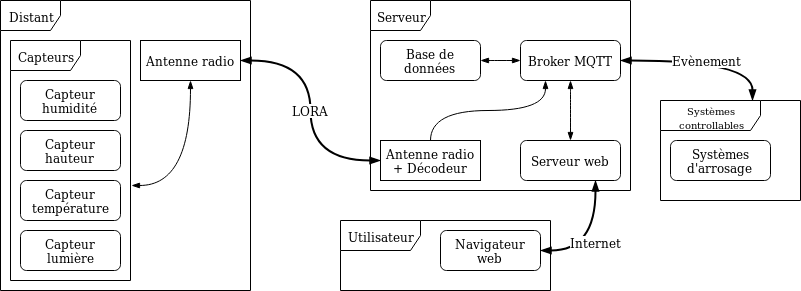
\includegraphics[scale=0.5]{graph.png}
	\end{centering}
	\caption{Infrastructure générale}
\end{figure}

\section{Résultats attendus}

\paragraph{}Les résultats attendus sont une gestion intelligente et automatisée des ressources, la première étant l'eau.
\paragraph{}Les interventions de l'utilisateur devront être minimes, tout en lui assurant des possibilités de contrôle et de surveillance des différents appareils de son exploitation.
\paragraph{}Le système doit, à partir d'un profil pré-configuré choisi par l'utilisateur, déclencher certaines actions, comme l'arrosage, et fournir à l'utilisateur une représentation claire des données ainsi que des analyses / prévisions.
\paragraph{}L'autonomie des capteurs doit leur permettre de fonctionner pendant au moins un an. Les capteurs doivent pouvoir communiquer avec les serveurs depuis une distance pouvant aller jusqu'à 3km. Chaque capteur doit transmettre des données toutes les dix minutes au moins.
\paragraph{}De nouveaux capteurs doivent facilement pouvoir être ajoutés au produit fini.

\end{document}
